\documentclass[a4paper]{article}
\usepackage{bbold}
\usepackage{amsmath}
\usepackage{tikz}
\title{Asymmetric sphere on a tilted slide}
\date{}
\begin{document}
\maketitle
\begin{figure}[h]
\centering
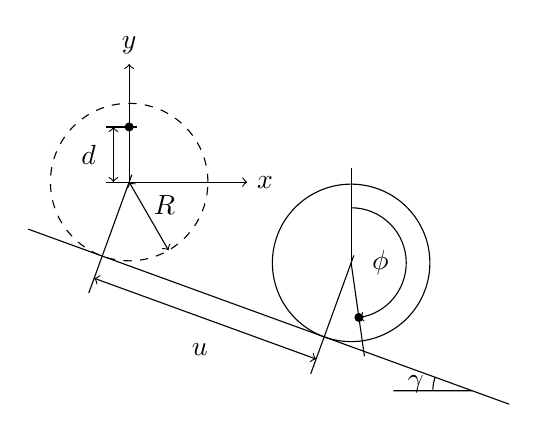
\begin{tikzpicture}
\draw[->] (0,0) -- (1.5,0) node[anchor=west] {$x$};
\draw[->] (0,0) -- (0,1.5) node[anchor=south] {$y$};
\begin{scope}[dashed]
    \draw (0,0) circle(1);
\end{scope}
\filldraw (0, .7) circle(.05);
\draw (-.3, .7) -- (.1,.7);
\draw (-.3, 0) -- (0,0);
\draw[<->] (-.2, 0) -- (-.2, .7);
\draw (-.3, .35) node[anchor=east] {$d$};
\draw[<->] (0, 0) -- (-60:1);
\draw (-50:.7) node[anchor=south] {$R$};

\begin{scope}[rotate=-20, yshift=-1cm]
    \draw (-1,0) --  (5.5,0);
    \draw (0, -.5) -- (0, 1.1);
    \draw (3, -.5) -- (3, 1.1);
    \draw[<->] (0, -.3) -- (3, -.3);
    \draw (1.5, -.5) node[anchor=north] {$u$};
    \draw (5,0) -- +(200:1);
    \draw (5,0) +(190:.5) node[anchor=east] {$\gamma$};
    \draw (4.5,0) arc(180:200:.5);
\end{scope}
\begin{scope}[rotate=-20, xshift=3cm, rotate=20]
    \draw (0,0) circle(1);
    \draw (0,0) -- (0,1.2);
    \draw (0,0) -- (-81.9:1.2);
    \filldraw (-81.9:.7) circle(.05);
    \draw[->] (0,.7) arc(90:-81.9:.7);
    \draw (.6,0) node[anchor=east] {$\phi$};
\end{scope}
\end{tikzpicture}
\end{figure}

\noindent Position of symmetry center
\begin{eqnarray*}
x_\mathrm{sym} &=& u \cos{\gamma} = R \phi \cos{\gamma}\\
y_\mathrm{sym} &=& -u \sin{\gamma} = -R \phi \sin{\gamma}
\end{eqnarray*}
Position of CoG
\begin{eqnarray*}
x_\mathrm{CoG} &=& x_\mathrm{sym} + d \sin{\phi} = R \phi \cos{\gamma} + d \sin{\phi}\\
y_\mathrm{CoG} &=& y_\mathrm{sym} + d \cos{\phi} = -R \phi \sin{\gamma} + d \cos{\phi}
\end{eqnarray*}
Linear velocity of CoG
\begin{eqnarray*}
v^2 &=& \dot{x}_\mathrm{CoG}^2 + \dot{y}_\mathrm{CoG}^2\\
&=& \dot{\phi}^2 \left( (R \cos{\gamma} + d \cos{\phi})^2 + (-R \sin{\gamma} - d \sin{\phi})^2 \right)\\
&=& (R^2 + d^2 + 2Rd \cos{\gamma} \cos{\phi} + 2Rd \sin{\gamma} \sin{\phi}) \dot{\phi}^2\\
&=& (R^2 + d^2 + 2Rd \cos(\phi - \gamma)) \dot{\phi}^2
\end{eqnarray*}
Total kinetic energy
\begin{eqnarray*}
T &=& \frac{1}{2} m v^2 + \frac{1}{2} I \omega^2\\
&=& \frac{1}{2} m (R^2 + d^2 + 2Rd \cos(\phi - \gamma)) \dot{\phi}^2
 + \frac{1}{2} I \dot{\phi}^2
\end{eqnarray*}
Total potential energy
\begin{eqnarray*}
V &=& mg y_\mathrm{CoG}\\
&=& -mgR \sin(\gamma) \phi + mgd \cos{\phi}
\end{eqnarray*}
Lagrange function
\begin{displaymath}
L = T - V
\end{displaymath}
Equation of motion
\begin{displaymath}
\frac{\mathrm{d}}{\mathrm{d}t} \frac{\partial L}{\partial \dot{\phi}}
- \frac{\partial L}{\partial \phi} = 0
\end{displaymath}
\begin{eqnarray*}
\frac{\partial L}{\partial \dot{\phi}} &=& m (R^2 + d^2 + 2Rd \cos(\phi - \gamma)) \dot{\phi} + I \dot{\phi}\\
\frac{\mathrm{d}}{\mathrm{d}t} \frac{\partial L}{\partial \dot{\phi}} &=&
m(R^2 + d^2 + 2Rd\cos(\phi - \gamma)) \ddot{\phi} + I \ddot{\phi}
- 2mRd \sin(\phi - \gamma) \dot{\phi}^2\\
\frac{\partial L}{\partial \phi} &=& -mRd \sin(\phi-\theta) \dot{\phi}^2
+ mgR \sin{\gamma} + mgd \sin{\phi}\\
\end{eqnarray*}
\begin{displaymath}
\ddot{\phi} = \frac{mRd \sin(\phi - \gamma) \dot{\phi}^2 + mgR \sin{\gamma} + mgd \sin{\phi}}
{m(R^2 + d^2 + 2Rd\cos(\phi - \gamma)) + I}
\end{displaymath}
\end{document}
